\chapter{Active Galactic Nuclei}
\label{chap:Background}
\section{General concepts}
As technology progressed through the 20th century, astronomers were able to observe the universe in new ways, discovering new phenomena and objects that were previously unknown. Discoveries such as the cosmic microwave background and pulsars revolutionized our understanding of the universe and the laws of physics that govern it.

The third discovery which is often mentioned in the same breath as these two is that of Active Galactic Nuclei (AGN), or more precisely, quasars ("Quasi stellar radio sources").

These objects are among the most luminous and energetic in the universe, being able to outshine entire galaxies in a volume which is incredibly small. The energy output of these objects is so high that it is difficult to explain how they can produce so much energy. The most accepted theory is that this energy is produced by the accretion of matter onto supermassive black holes which have masses ranging anywhere from $10^6$ to $10^10$ solar masses. The matter is heated up to millions of degrees, and the radiation produced is emitted across the electromagnetic spectrum, through different processes.

The structure of AGNs is complex, with different regions emitting different types of radiation. Generally, we find the following:

\begin{itemize}
    \item \textbf{The Supermassive Black Hole:} A black hole whose origins are still debated, but which is believed to have formed in the early universe. It has a mass of $10^6 - 10^{10}$ solar masses, and is the source of the energy produced in AGNs.
    \item \textbf{The Accretion Disk:} A disk of matter orbiting the black hole, gradually being accreted onto it. The matter in the disk is heated to millions of degrees, emitting radiation across the electromagnetic spectrum.
    \item \textbf{The Corona:} A region of hot, ionized gas located beyond the accretion disk, believed to be the source of X-ray emission in AGNs.
    \item \textbf{The Obscuring Torus:} A region of dust and gas surrounding the accretion disk, which absorbs some of the radiation and re-emits it in the infrared.
    \item \textbf{The Broad Line Region:} A region of ionized gas composed of numerous small, rapidly moving clouds situated near the accretion disk. This region emits broad emission lines in the optical and ultraviolet spectrum due to the Doppler effect caused by the high velocities.
    \item \textbf{The Narrow Line Region:} A region of ionized gas located further away from the accretion disk, which emits narrow emission lines in the optical and ultraviolet spectrum. The narrowness of these lines is due to the lower velocities of the gas clouds.
    \item \textbf{The Jet:} Some AGN present a region of highly energetic particles that are ejected from the poles of the black hole at relativistic speeds. These jets can extend for thousands of light-years and emit all kinds of radiation.
\end{itemize}

The figure below illustrates neatly the structure of an AGN.

\begin{figure}[H]
    \centering
    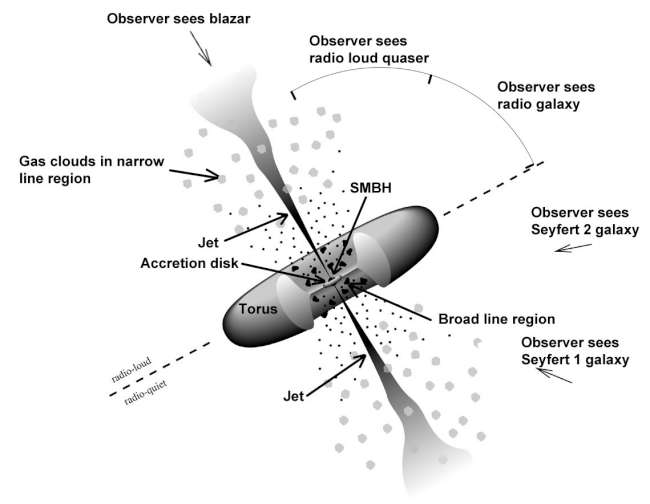
\includegraphics[width=0.7\textwidth]{Figures/AGN Structure.jpg}
    \caption{The structure of an Active Galactic Nucleus. The different regions mentioned before are labeled.}
    \label{fig:AGN_structure}
\end{figure}


\section{The AGN of NGC 1068}

The AGN of NGC 1068 is one of the most studied AGNs in the night sky, being relatively close to us (14.4 Mpc) and having a high luminosity. It is classified as a Seyfert II galaxy, which means that it has a bright nucleus and narrow emission lines in its spectrum. The AGN of NGC 1068 is known for its complex structure, with a large amount of gas and dust surrounding the nucleus, which makes it difficult to observe in the optical and ultraviolet spectrum.

The AGN of NGC 1068 has been observed across the electromagnetic spectrum, from radio to gamma rays. The gamma-ray emission of this AGN is particularly interesting, as it has been detected by the \textit{Fermi} satellite and the MAGIC telescope. The gamma-ray emission of NGC 1068 is believed to be produced by the interaction of high-energy particles with the gas and radiation in the AGN, leading to the production of gamma rays through different processes.

\section{Radiation}

%The background section should give sufficient background information to give the reader an overview of the state-of-the-art research field in which you work.

%The background chapter can be a bit similar to the introduction. For journal articles, it is not that common with a background section, as it is not kept separate from the introduction. However, for a master thesis, it is common to have more background and therefore to separate out some of the background material into a separate chapter. For a specialization project, the background chapter could be the most important chapter, as the specialization project is centered around learning a new subject field.

%Do not overestimate the background knowledge of the reader. As a rule of thumb, you could assume (s)he knows as much as you did when you started on your master thesis/project. So you need to give the reader enough background to be able to read the rest of your thesis.

%All relevant literature should be included, so do a thorough literature search. When you do, try not to miss out on the classics and defining papers in your field of work. For a specialization project, your background section can include references to display the breadth of the field you are working on. In contrast, for a master thesis, you should be able to argue for all included references. Do not add references just to get a long reference list. After you have spent a lot of time reading something, it could be tempting to add those references to just show off that you have read them, even though it turned out after reading them that it is not fully related to your work. Do not, all included references in your master thesis should be relevant to your work.

%The background material should also motivate your work. It should make your research question interesting by showing what others have done, and showing what is missing, highlighting the void that you try to fill with your work.


%\section{Citations}

%The background needs relevant literature to place your project work into context. The Google-scholar search (\url{scholar.google.com}) is a good starting point for searching for relevant papers.  This subsection will show how to include these references in your latex-document.

%There is a long range of different styles and packages in Latex for citations. During your writing process, it is often beneficial to have an \texttt{authoryear} style, where you see the author(s) and the year of publication. This will help you remember what the reference is. In the \texttt{main.tex} file you will find a command defining the bibliography style.

%This is where you want to go to change the style of your referencing. In this setup, we use the \texttt{natbib} style. This allows for using \verb=\citep= and \verb=\citet= references, which are useful if you use \texttt{authoryear} style:
%\begin{itemize}
 %   \item Whenever the reference is part of the sentence, you should use the textual citation \verb=\citet=. The \verb=\citet= reference types will give a reference that looks like this: \citet{berg2014permeability}.
 %   \item Whenever the reference is not a part of the sentence, but just general for the sentence or paragraph, you should use the parenthetical citation \verb=\citep=. The \verb=\citep= reference types will give a reference that looks like this: \citep{berg2014permeability}.
 %   \item If you do not specify, but use \verb=\cite=, it will look like this: \cite{berg2014permeability}.
%\end{itemize}

%All the references you use will automatically show up in your reference list. If you want to shift to numerical citations, you should use the \texttt{cite} command, as there are no differences between textual and parenthetical citations when you use the numerical style.